%! Correction + grammar & writing check for Background up to Regression
\chapter{Theory \& Methodological Background}
\label{sec:background}
This chapter provides an overview of the theoretical background used in this thesis. While the focus of this thesis is set on the application of machine learning methods within a quantum chemistry context, a basic introduction to computational quantum chemistry methods, in particular self-consistent field (SCF) methods, is provided. 

\section{Self-consistent Field (SCF) Theory}
\label{sec:background_scf}
Quantum chemistry has its roots far before the advent of the computer age. Based on the original theories on quantum mechanics formulated by Schrödinger and Heisenberg, the interest in the accurate description of matter via this new theory was sparked. After the introduction of the wavefunction by Schrödinger almost a century ago, Max Born's statistical interpretation enabled a direct calculation of the electron density. \parencite{ref:schroedinger_1926undulatory} Already a year later, Hartree coined a self-consistent method to solve the many-electron problem utilizing a mean-field approach. Slater and Fock independently adapted the method by adding the exchange term and consistency with the Pauli exclusion principle. This method was later named Hartree-Fock (HF) method. \parencite{ref:Hartree_1928,ref:slater1930note,ref:fock1930naherungsmethode} From that point on many advancements have been made in this field. Most prominently density functional theory (DFT), coupled cluster methods (CC), and pertubative expansions (MP2) have been developed. Yet, the theory behind the HF method is still the foundation for nearly all of these methods.

The following introductory overview of the Hartree-Fock method is mostly based on the book by Szabo and Ostlund. \parencite{ref:szabo_ostlund}

\subsection{Foundations and Formalism of the Hartree-Fock Method}
\label{subsec:background_hf}
The Born Oppenheimer approximation allows for a separate treatment of the nuclear and electronic problem of a system. This is motivated by the vastly different masses and hence different time scales of nuclei and electron movement. The total wavefunction of a system may be written as a product state of electronic and nuclear wavefunctions (using the convention of small letters for electrons and capital letters for nuclei coordinates):
\begin{equation}
    \Psi_{\text{tot}}(\mathbf{r}_n, \mathbf{R}_m) = \Psi_{\text{elec}}(\mathbf{r}_n; \mathbf{R}_m) \Psi_{\text{nuc}}(\mathbf{R}_m)
\end{equation}
Using our approximation, the nuclear wavefunction can be obtained rather easily by solving the nuclear Schrödinger equation for an effective potential which corresponds to the electronic energy written as a function of nuclear coordinates.  
Within the confines of this thesis, we will focus on the electronic wavefunction as a prerequisite, and therefore omit the subscript from here on. It parametrically depends on the nuclear coordinates and is the solution to the time independent Schrödinger equation:
\begin{equation}
    H \Psi(\mathbf{r}_n; \mathbf{R}_m) = E[\Psi](\mathbf{R}_m) \Psi(\mathbf{r}_n; \mathbf{R}_m)
\end{equation}
The electronic energy $E$ is a functional of the electronic wavefunction. We will minimize this energy using orthogonality constraints on the wavefunction, as will be explained later. Written in atomic units, the corresponding Hamiltonian operator $H$ for $N$ electrons and $M$ nuclei reads
\begin{equation}
    H = T + V_{\text{ne}} + V_{\text{ee}} = -\frac{1}{2} \sum_{i=1}^N \nabla_i^2 - \sum_{i=1}^N \sum_{A=1}^M \frac{Z_A}{|\mathbf{r}_i - \mathbf{R}_A|} + \sum_{i<j}^N \frac{1}{|\mathbf{r}_i - \mathbf{r}_j|}.
\end{equation}
Note that we do not include kinetic or repulsion terms for the nuclei as we are only considering the electronic problem. The first term is the kinetic energy operator, the second term describes the interaction of the electrons with the nuclei, and the last term describes the electron-electron interaction.

With electrons being fermions, we have to take antisymmetrization into account. Mathematically, this can be achieved by writing the wavefunction as a determinant, which ensures parity change under exchange of two rows\footnote{Furthermore, if two electrons occupy the same orbital the determinant will vanish.}. For $N$ electrons this can be written as:
\begin{equation}
    \Psi(\mathbf{x}_1, \mathbf{x}_2, \ldots, \mathbf{x}_N) = \frac{1}{\sqrt{N!}}
    \begin{vmatrix}
    \chi_1(\mathbf{x}_1) & \chi_2(\mathbf{x}_1) & \cdots & \chi_N(\mathbf{x}_1) \\
    \chi_1(\mathbf{x}_2) & \chi_2(\mathbf{x}_2) & \cdots & \chi_N(\mathbf{x}_2) \\
    \vdots & \vdots & \ddots & \vdots \\
    \chi_1(\mathbf{x}_N) & \chi_2(\mathbf{x}_N) & \cdots & \chi_N(\mathbf{x}_N)
    \end{vmatrix}
\end{equation}
To write down this so-called Slater determinant we have introduced the notation $\mathbf{x}_i = (\mathbf{r}_i, \omega_i)$ with $\omega_i$ being the spin coordinate of electron $i$. The functions $\chi_i$ are called spin orbitals and are a product of spatial and spin functions. 
% \begin{equation}
%     \label{eq:spin_orbital_expansion}
%     \chi_i(\mathbf{x}) = \sum_{\nu} C_{\nu i} \chi_\nu(\mathbf{x}) = \sum_{\nu} C_{\nu i} \phi_\nu(\mathbf{r}) \sigma(\omega) \text{ with } \bra{\chi_i}\ket{\chi_j} = \delta_{ij} \text{ and } \sigma(\omega)=
%   \bigl\{\begin{smallmatrix}
%     \uparrow \text{ for } \omega =&\nicefrac{1}{2}\\
%     \downarrow  \text{ for } \omega =& -\nicefrac{1}{2}
%   \end{smallmatrix}\bigr.
% \end{equation}

\begin{equation} %FRAGE weche Notation ist klarer? 
  \label{eq:spin_orbital_expansion}
  \chi_i(\mathbf x) = \sum_{\nu} C_{\nu i}\,\chi_\nu(\mathbf x) = \sum_{\nu} C_{\nu i}\,\phi_\nu(\mathbf r)\,\sigma(\omega), \quad
  \langle\chi_i|\chi_j\rangle = \delta_{ij},  \quad
  \sigma(\omega) =
    \begin{cases}
      \alpha(\omega)&\text{if }\omega=+\tfrac12\\
      \beta(\omega)&\text{if }\omega=-\tfrac12\\
      0&\text{otherwise}
    \end{cases}
\end{equation}
Here, spin functions use the common notation $\alpha(\omega)$ and $\beta(\omega)$ for spin up and down respectively.
Using this expansion, we reduce the problem to the determination of the coefficients $C_{\nu i}$ for a given set of orthogonal basis functions $\phi_\nu(\mathbf{r})$. For a complete set of basis functions this expansion is exact. However, in practice, we have to limit the number of basis functions and hence the size of our Slater determinant to a computationally feasible size. For the subsequent considerations we introduce the shorthand ket for a slater determinant $\ket{\Psi} = \ket{\chi_1, \chi_2, \ldots, \chi_N}$ or $\ket{\Psi} = \ket{1, 2, \ldots, N}$ for the sake of brevity.

%Energy functional
A slater determinant is one simple way of describing the state of a system as a linear combination of basis functions. From that we can derive the energy of the given systems state $E$ using
\begin{equation}
    \label{eq:elec_energy}
    E[\Psi] = \bra{\Psi} H \ket{\Psi}.
\end{equation}
For our considerations we will be interested in the ground state of the system. This means we need to find the minimum of our energy functional $E[\Psi]$ and its corresponding slater determinant $\ket{\Psi}$, which marks our approximation to the ground state wavefunction. This is done via the variational principle, which yields an eigenvalue problem,
\begin{equation}
    \label{eq:hf_eigenval_equation}
    F \ket{\Psi_i} = \varepsilon_i \ket{\Psi_i},
\end{equation}
called the Hartree-Fock (HF) equations. Here $\varepsilon_i$ corresponds to the energy of the $i$-th spin-orbital $\ket{\Psi_i}$. The operator $F$ is called the Fock operator and is defined as an effective one electron operator acting on electron coordinate $i$:
\begin{equation}
    F(i) = 
    \underbrace{
        -\frac{1}{2} \nabla^2 
        - \sum_{A=1}^M \frac{Z_A}{|\mathbf{r} - \mathbf{R}_A|}
    }_{\text{core Hamiltonian } h(i)}
    + 
    \underbrace{
        \sum_{j\neq i} J_j(i) - K_j(i).
    }_{\text{HF potential }v^{HF}(i)}
\end{equation}
While the core Hamiltonian $h(i)$ contains the well-known kinetic and nuclear attraction terms, the Hartree-Fock potential $v^{HF}(i)$ condenses all electron-electron interaction into a mean-field effect on electron $i$ using the Coulomb and exchange terms,
\begin{subequations}
\begin{align}
    J_j(i)\chi_i(\mathbf{x}_1) &= \left[ \int d\mathbf{x}_2\, \frac{|\chi_j(\mathbf{x}_2)|^2}{r_{12}} \right] \chi_i(\mathbf{x}_1),\\
    K_j(i)\chi_i(\mathbf{x}_1) &= \left[ \int d\mathbf{x}_2\, \frac{\chi_j^*(\mathbf{x}_2)\chi_i(\mathbf{x}_2)}{r_{12}} \right] \chi_j(\mathbf{x}_1).
\end{align}
\end{subequations}
Here, $J_j(i)$ is the Coulomb operator, representing the classical electrostatic repulsion, and $K_j(i)$ is the exchange operator, arising from the antisymmetry of the wavefunction.

While \autoref{eq:hf_eigenval_equation} seems like an ordinary eigenvalue problem, the $\chi$ terms in $J$ and $K$ depend on our slater determinant wavefunction $\ket{\Psi}$. Thus, to get the ground state wavefunction, we need the corresponding Fock operator $F$, which in turn depends on the ground state wavefunction. 

%DONE

\subsection{Matrix formulation of the Hartree-Fock equations}
\label{subsec:background_hf_computational}
To solve the self-dependence of the Hartree-Fock equations, we need to iteratively update our wavefunction until convergence is reached. To achieve this we first need to express our eigenvalue problem in a way that can be solved numerically. Assuming each spin up ($\uparrow$) and spin down ($\downarrow$) electron pair occupies the same spatial orbital (referred to as restricted HF), we can write the HF-equations for electron 1 as follows:
\begin{equation}
    F(\mathbf{x}_1) \chi_i(\mathbf{x}_1) = \varepsilon_i \chi_i(\mathbf{x}_1) \equiv F(\mathbf{x}_1) \psi_i(\mathbf{r}_1) \sigma_i(\sigma_1) = \varepsilon_i \psi_i(\mathbf{r}_1) \sigma_i(\sigma_1).
\end{equation}
With the spins integrated out, we obtain the HF-equations for spatial orbitals, 
\begin{equation}
    \label{eq:hf_eigenval_equation_spatial}
    F(\mathbf{r}_1) \psi_i(\mathbf{r}_1) = \varepsilon_i \psi_i(\mathbf{r}_1),
\end{equation}

which differs from \autoref{eq:hf_eigenval_equation} in the fact that we have integrated out the spin degrees of freedom and thus need to sum over half the electrons (i.e. $\uparrow$) and double the result, reflecting the closed-shell assumption that all spins are paired. With this, the Fock operator takes the form 
\begin{equation}
    \label{eq:fock_operator_spatial}
    F(\mathbf{r}_1) = h(\mathbf{r}_1) + 2 \sum_{j\neq i}^{\nicefrac{N}{2}} \left( J_j(\mathbf{r}_1) - K_j(\mathbf{r}_1) \right).
\end{equation}

We need to represent the spatial orbitals in a finite, computer-readable way. While the spatial orbitals in \autoref{eq:spin_orbital_expansion} are exact for a complete basis set, we will limit ourselves to a finite set of known basis functions, which will approximate the spatial orbitals by a linear combination.
\begin{equation}
    \label{eq:psi_approximation}
    \psi_i(\mathbf{r}) \approx \sum_{\nu}^{K} C_{\nu i} \phi_\nu(\mathbf{r})
\end{equation}
%! start new content
Possible ways to construct a finite set of basis functions $\phi_\nu(\mathbf{r})$ to represent the spatial orbitals $\psi_i(\mathbf{r})$ are introduced in \autoref{subsec:background_hf_basis_sets}. \\
Given this finite set of equations, we can now find an expression in matrix form to make it suitable for numerical solution.
Substituting \autoref{eq:psi_approximation} into \autoref{eq:hf_eigenval_equation_spatial} yields
\begin{equation}
    \label{eq:roothhaan_intermediate_1}
    F(\mathbf{r_1}) \sum_{\nu}^{K} C_{\nu i} \phi_\nu(\mathbf{r_1}) = \varepsilon_i \sum_{\nu}^{K} C_{\nu i} \phi_\nu(\mathbf{r_1}).
\end{equation}
We multiply both sides by $\phi_\mu^*(\mathbf{r_1})$ and integrate over the spatial coordinate $\mathbf{r_1}$ to get
\begin{equation}
    \label{eq:roothaan_equations}
        \sum_{\nu}^{K} C_{\nu i} \underbrace{\int d\mathbf{r_1} \phi_\mu^*(\mathbf{r_1}) F(\mathbf{r_1}) \phi_\nu(\mathbf{r_1})}_{F_{\mu\nu}} = \varepsilon_i \sum_{\nu}^{K} C_{\nu i} \underbrace{\int d\mathbf{r_1} \phi_\mu^*(\mathbf{r_1})\phi_\nu(\mathbf{r_1})}_{S_{\mu\nu}}.
\end{equation}
Now we define the matrix elements for the Fock matrix $\mathbf{F}$ and the overlap matrix $\mathbf{S}$ using
\begin{subequations}
    \label{eq:roothaan_matrices}
    \begin{align}
        F_{\mu \nu} &= \int d\mathbf{r_1} \phi_\mu^*(\mathbf{r_1}) F(\mathbf{r_1}) \phi_\nu^*(\mathbf{r_1}), \label{eq:roothaan_mat_F}\\
        S_{\mu \nu} &= \int d\mathbf{r_1} \phi_\mu^*(\mathbf{r_1}) \phi_\nu^*(\mathbf{r_1}),
    \end{align}
\end{subequations}
so that the eigenvalue problem writes:
\begin{subequations}
    \begin{align}
        \sum_{\nu}^{K} F_{\mu\nu} C_{\nu i}  &= \varepsilon_i \sum_{\nu}^{K} S_{\mu\nu} C_{\nu i},\\
        \mathbf{FC} &= \mathbf{SC} \boldsymbol{\varepsilon}.    \label{eq:roothaan_equations_matrix}
    \end{align}
\end{subequations} 
In \autoref{eq:roothaan_equations_matrix} $\boldsymbol{\varepsilon}$ is a diagonal matrix with the orbital energies $\varepsilon_i$ on the diagonal and $\mathbf{C}$ is the matrix of the expansion coefficients $C_{\nu i}$. This equation is called the Roothaan equations and can be solved iteratively. \\
Yet, we still are missing a representation of the density in terms of the expansion coefficients $C_{\nu i}$ and the basis functions $\phi_\nu(\mathbf{r})$. The probability to find an electron at a certain position $\mathbf{r}$ is given by the square of the wavefunction $\psi_i(\mathbf{r})$ and thus the electron density $\rho(\mathbf{r})$ can be written as
\begin{equation}
    \rho(\mathbf{r}) = 2 \sum_{i=1}^{\nicefrac{N}{2}} |\psi_i(\mathbf{r})|^2 = 2 \sum_{i=1}^{\nicefrac{N}{2}} \sum_{\mu,\nu}^{K} C_{\mu i} C_{\nu i}^* \phi_\mu(\mathbf{r}) \phi_\nu^*(\mathbf{r}) = \sum_{\mu,\nu}^{K} P_{\mu \nu} \phi_\mu(\mathbf{r}) \phi_\nu^*(\mathbf{r}).
\end{equation}
Here we have used \autoref{eq:psi_approximation} to express the spatial orbitals in terms of the basis functions\footnote{We still need to multiply by two in order to account for spin up and spin down.} and defined the density matrix $\mathbf{P}$ with matrix elements
\begin{equation}
    \label{eq:density_matrix}
    P_{\mu \nu} = 2 \sum_{i=1}^{\nicefrac{N}{2}} C_{\mu i} C_{\nu i}^*.
\end{equation}
As we have seen earlier, the Fock operator $F$ and thus the Fock matrix $\mathbf{F}$ depend on the expansion coefficients $\mathbf{C}$ and thus the Fock matrix also depends on the density matrix $\mathbf{F(P)}$. If we insert \autoref{eq:fock_operator_spatial} into \autoref{eq:roothaan_mat_F} and write out Coulomb and exchange terms we have: 
\begin{align}
    \label{eq:fock_full_eq_coul_ex}
        F_{\mu \nu} &= \underbrace{\int d\mathbf{r}_1\, \phi_\mu^*(\mathbf{r}_1)\, h(\mathbf{r}_1)\, \phi_\nu(\mathbf{r}_1) \nonumber}_{H_{\mu\nu}^\text{core}} \\
        &\quad + \sum_{\lambda \sigma} \mathbf{P}_{\lambda \sigma} \Bigg[
            \underbrace{\iint  d\mathbf{r}_1 d\mathbf{r}_2\, \phi_\mu^*(\mathbf{r}_1) \phi_\nu(\mathbf{r}_1) r_{12}^{-1} \phi_\sigma^*(\mathbf{r}_2) \phi_\lambda(\mathbf{r}_2) \nonumber}_{\text{Coulomb-term}} \\
            &\qquad - \frac{1}{2} \underbrace{\iint d\mathbf{r}_1 d\mathbf{r}_2\, \phi_\mu^*(\mathbf{r}_1) \phi_\lambda(\mathbf{r}_1) r_{12}^{-1} \phi_\sigma^*(\mathbf{r}_2) \phi_\nu(\mathbf{r}_2)}_{\text{Exchange-term}}
            \Bigg]
\end{align}
One and two electron contributions are now split into the core Hamiltonian $H_{\mu\nu}^\text{core}$ term, which is independent of the density matrix and thus stays constant for a given set of basis functions, and the Coulomb and exchange terms that depend on the density matrix $\mathbf{P}$. The latter terms are often denoted as $G_{\mu\nu}$, the so-called two-electron integrals, hence $F_{\mu \nu} = H_{\mu\nu}^\text{core} + G_{\mu\nu}$.

\subsection{The Self-Consistent Field (SCF) Algorithm}
\label{subsec:background_hf_scf}
We now have all ingredients to solve \autoref{eq:roothaan_equations_matrix} iteratively. The self-consistent field (SCF) algorithm is a fixed-point iteration method: it starts from an initial density guess and then alternates between building the Fock matrix and updating the density until convergence. To generate the initial guess, we must supply the molecular geometry $\{\mathbf R_A, Z_A\}$, the total electron count $N$, and a chosen basis set $\{\phi_\nu\}$ to represent our orbitals.\\

Initially, we calculate the core Hamiltonian $H_{\mu\nu}^\text{core}$ and the overlap matrix $S_{\mu\nu}$ once (they will be reused in every step) and we guess an initial density. The guess of this initial density is crucial and has a big effect on the convergence of the algorithm. Then we start the loop: 
\begin{enumerate}[itemsep=0.1em]
    \item Calculate $G_{\mu\nu}$ using the current $\mathbf{P}$.
    \item Build a new $\mathbf{F}$ using $H_{\mu\nu}^\text{core}$ and $G_{\mu\nu}$.
    \item Solve the generalized eigenvalue problem\footnote{For numerical stability one usually converts to a standard eigenproblem using canonical orthonormalization: diagonalize $\mathbf{S}=\mathbf{U}\,s\,\mathbf{U}^T$, form $\mathbf{X}=\mathbf{U}\,s^{-1/2}$, solve the standard problem $\mathbf{X}^T\mathbf{F}\,\mathbf{X}\,\mathbf{C}'=\mathbf{C}'\,\boldsymbol{\varepsilon}$, and recover $\mathbf{C}=\mathbf{X}\,\mathbf{C}'$.} to obtain a new $\mathbf{C}$ and $\boldsymbol{\varepsilon}$. 
    \item Obtain a new density matrix $\mathbf{P}$ from the new $\mathbf{C}$.
    \item Total energy or $\mathbf{P}$ converged? If not, repeat.
\end{enumerate}

Computationally, the calculation of the two-electron integrals $G_{\mu\nu}$ is the most expensive step which scales with the number of basis functions as $\bigO{K^4}$. Given this fact, a small enough basis set that still captures the essence of the physical system, should be chosen and the number of iterations shall be kept to a minimum by a good initial guess. Keeping our approximations of the spatial orbitals via \autoref{eq:psi_approximation} in mind, we see that better approximations of the electronic wavefunction and its corresponding energy can be achieved with larger basis sets. Given the drawback of increased computational cost (mostly in the first step of the SCF algorithm), a reduction of iterations is even more crucial for larger systems and larger basis sets.
\subsection{Guessing schemes}
\label{subsec:background_hf_guessing}
As eluded to earlier, our algorithm needs an initial density matrix $\mathbf{P}$ to start the SCF iteration. Over the years various schemes have been developed and implemented in quantum chemistry packages. It is instructive to introduce two commonly used schemes here. For sake of brevity, details regarding initial guess strategies in PySCF can be found in \autoref{sec:appendix}.\\

\textbf{Superposition of Atomic Densities (SAD) / Minimal Atomic Orbital (MINAO)}\\
This scheme builds on atomic HF calculations, which are performed for each element appearing in a given molecule. With very little overhead, these calculations yield initial atomic densities, usually calculated in a minimal atomic basis, which are expanded into the molecular basis and used to build an initial block diagonal density matrix. After calculating the Fock matrix from this density, one diagonalizes it to obtain the molecular orbitals. Although the initial density matrix is strictly block-diagonal, diagonalizing the Fock matrix naturally mixes atomic orbitals and generates non-zero off-block elements. \parencite{ref:sad_guess}

\textbf{Generalized Wolfsberg-Helmholtz (GWH)}\\
A semi-empirical approach is given by the generalized Wolfsberg-Helmholtz method. It approximates the off-diagonal elements of the core Hamiltonian from the diagonal values, weighting them according to orbital overlap,
\begin{equation}
    \label{eq:gwh}
    F_{ij} \approx H^{\text{core}}_{ij} = \frac{K}{2}(H^{\text{core}}_{ii} + H^{\text{core}}_{jj})S_{ij},
\end{equation}
where $K$ is a constant usually set to $1.75$. From \autoref{eq:fock_full_eq_coul_ex} it is immediately evident that this approximation completely omits Coulomb and exchange terms, reducing the Fock matrix to core-Hamiltonian integrals evaluated with the same orbitals on both sides. \parencite{ref:gwh_wolfsberg1952spectra, ref:Lehtola2019}

\subsection{Expectation values}
\label{subsec:background_hf_derived_quantities}
Several quantities can be derived from the solution of the Hartree-Fock equations. As eluded to in \autoref{eq:hf_eigenval_equation}, the eigenvalues of $F$ are treated as orbital energies $\varepsilon_i$. 
The lowest $\nicefrac{N}{2}$ eigenvalues correspond to the occupied orbitals, while the rest are so-called virtual orbitals \footnote{We still assume closed shell systems with equal number of spin up and spin down electrons.}. One might be tempted to simply sum over the occupied orbital energies to obtain the total energy of the system. However, this leads to a double counting of the energy given by the exchange interaction for electron pairs. The correct electronic energy needs to be evaluated by calculating
\begin{equation}
    \label{eq:elec_energy_hf_gs}
    E^\text{HF}_0 =  \bra{\Psi^\text{HF}_0} H \ket{\Psi^\text{HF}_0},
\end{equation}
with $\Psi^\text{HF}_0$ denoting the HF ground state wavefunction built from the $\nicefrac{N}{2}$ lowest energy orbitals.
Furthermore, the orbital energies can be used to estimate ionization energies in a frozen shell model, as stated by Koopmans' theorem. \parencite{ref:koopmans1934} Removing an electron from an occupied orbital $\chi_i$ will lead to an increase in energy of $\varepsilon_i$.

By inserting $F$ for the Hamiltonian in \autoref{eq:elec_energy}, one directly derives the total energy of the closed-shell ground state: 
\begin{subequations}
\begin{align}
    E^\text{HF}_0 &= \bra{\Psi^\text{HF}_0} H \ket{\Psi^\text{HF}_0} = 2\sum_{i=1}^{\nicefrac{N}{2}} \bra{\chi_i} h(i) \ket{\chi_i}
    + \frac{1}{2}\sum_{i=1}^{\nicefrac{N}{2}}\sum_{j=1}^{\nicefrac{N}{2}} \left[ 2 J_j(i) - K_j(i) \right]\\
    \implies E^\text{HF}_0 &= \sum_{i=1}^{\nicefrac{N}{2}}\left[ h(i) + \varepsilon_i\right] \text{  with  } \varepsilon_i = F_i =  h(i) + \sum_{j}^{\nicefrac{N}{2}} \left[ 2 J_j(i) - K_j(i) \right]\\
    \implies E^\text{HF}_0 &= \frac{1}{2} \sum_{\nu, \mu} P_{\mu \nu} \left[ H_{\mu \nu}^\text{core} + F_{\mu \nu} \right] = \frac{1}{2} \text{Tr} \left( \mathbf{P} \left[ \mathbf{H}^\text{core} + \mathbf{F} \right] \right)
\end{align}
\end{subequations}
To get the total energy of the system, one adds the nuclear repulsion energy 
\begin{equation}
E_\text{nuc} = \sum_{A<B} \frac{Z_A Z_B}{|\mathbf{R}_A - \mathbf{R}_B|}
\end{equation}
to the electronic energy $E^\text{HF}_0$, yielding the total energy of the system. Additionally, particularly from a chemical point of view, the number of electrons assigned to each atom is of interest, since partial charges can be derived from it. Given the fact that the density matrix represents spatial orbitals in the atom centred basis set, we can interpret $\mathbf{(PS)}_{\mu \mu}$ as the population of electrons on orbital $\mu$. This leads to a possible definition of a partial charge at atom $A$,
\begin{equation}
    q_A = Z_A - \sum_{\mu \in A} \mathbf{(PS)}_{\mu \mu},
\end{equation}
with index $\mu$ running over all basis functions located at atom $A$. This represents one of several approaches to population and charge analysis, commonly referred to as Mulliken population analysis. \parencite{ref:mulliken1955electronic}
\subsection{Basis sets}
\label{subsec:background_hf_basis_sets}
For computational treatment, our abstract basis functions $\phi_\nu(\mathbf{r})$ need to manifest in a concrete form. 
Motivated by the analytical solution of the Hydrogen atom, one can introduce so-called Slater-type orbitals (STOs) using an exponential radial term and spherical harmonics: \footnote{For sake of clarity the spherical harmonics term is written with $\Omega$ instead of $\theta$ \& $\varphi$.}
\begin{equation}
    \label{eq:slater_orbital}
    \phi_{n, l, m}^{\text{STO}}(r, \Omega, \zeta) = N Y_{l,m}(\Omega) r^{n-1} e^{-\zeta r}
\end{equation} 
Computationally, the integrals that occur by using linear combinations of STOs are expensive to calculate. 
\newpage
\textbf{Gaussian-Type Orbitals (GTOs)}\\
To circumvent this problem, one approximates STOs using contractions of Gaussian-type orbitals (GTOs), which have a Gaussian $e^{-\zeta r^2}$ in place of the Slater exponential $e^{-\zeta r}$. A GTO is defined as: 
\begin{equation}
    \label{eq:gaussian_orbital}
    \phi_{n, l, m}^{\text{GTO}}(r, \Omega, \zeta) = N Y_{l,m}(\Omega) r^{n-1} e^{-\zeta r^2}
\end{equation}
A linear combination of $N$ GTOs to approximate a STO is referred to as a contracted Gaussian function (CGF). We choose the contraction coefficients $c_i$ and the exponents $\zeta_i$ such that the CGF approximates the STO as closely as possible. \\
\begin{equation}
    \phi_{n, l, m}^{\text{STO}}(r, \Omega, \zeta)  \approx \phi_{n, l, m}^{\text{CGF}}(r, \Omega, \zeta) = \sum_{i=1}^N c_i \phi_{n, l, m}^{\text{GTO}_i}(r, \Omega, \zeta_i)
\end{equation}
Many basis sets with varying number of CGFs have been developed over the years, some common ones from the STO-nG family include STO-3G, STO-6-31G or STO-6-31G(2df,p). The n in this nomenclature of Pople type basis sets \parencite{ref:pople_basis} denotes the number of GTOs used in the contraction. While STO-3G uses three GTOs for each orbital, STO-6-31G uses six GTOs for the inner shell and two functions with three and one GTO respectively for the outer shell. Basis sets using more than one contracted function (31 in 6-31G) are so-called double-zeta basis sets; in this particular case it is a split-valence double zeta basis set because the core orbitals (6 in 6-31G) are modelled with only one contraction. The notation in parentheses denotes additional functions, e.g. STO-6-31G(2df,p)\footnote{also referred to as 6-31G(2df,p) in this thesis} uses two additional d-functions and one f-function on heavy atoms (\ch{C}, \ch{O}, \ch{N} \& \ch{F}). 

\textbf{Segmented Contraction}\\
Generally, the GTOs used in the contraction of Pople type basis sets are not reused and thus of the segmented contraction type. In contrast, general contraction type basis sets (such as cc-pVXZ \parencite{ref:cc-pVXZ}) reuse some or all primitives in multiple contractions. The latter can be converted to a computationally more efficient segmented form, which retains the initial accuracy. One such modern segmented basis family optimized for density functional theory are the pcseg-n basis sets. \parencite{ref:Jensen2014pcs}

\textbf{Accuracy \& Hartree Limit}\\
Expanding the spatial orbitals using basis functions introduces an error in the electron density distribution and subsequently the converged Energy $E_{HF}$. Given the limitation of a longer runtime-scaling with $\bigO{K^4}$ in the number of basis functions, the accuracy can be refined using a larger and more complete basis set. The so-called Hartree limit constitutes the lowest energy asymptotically attainable by any HF-calculation, achievable only with an infinitely large basis set. This can be estimated by the shrinking differences of energies obtained in a series of calculations with basis sets of increasing size. \parencite{ref:Jensen2005hf} Yet, it still lacks the correlation energy of electrons, and is therefore only of academic interest. We will discuss methods that build or improve on Hartree Fock next. 
\newpage
\subsection{Post-Hartree-Fock Methods}
\label{subsec:background_post_hf}
HF theory provides a solid foundation to solve the many-electron problem and is usually used as the starting point for following improvements. These are generally bundled under the umbrella term of post-Hartree-Fock methods.

\textbf{Configuration Interaction (CI)}\\
Configuration Interaction (CI) improves upon the Hartree-Fock approximation by expressing the many-electron wavefunction as a linear combination of multiple Slater determinants, including excited configurations. While HF provides the best single-determinant approximation to the ground state, it neglects electron correlation. CI systematically includes this by mixing determinants generated from excitations out of the HF reference, thus recovering the missing correlation energy. Combinatorially, for a system with $2K$ spin orbitals and $N$ electrons, the number of possible determinants grows as $\binom{2K}{N}$, which makes CI calculations, using all possible determinants (full CI) intractable for all but the smallest molecular systems. The number of determinants is usually limited by calculating only single and double excitations (CISD), resulting in a time complexity of $\bigO{K^6}$.

\textbf{Coupled Cluster (CC)}\\
Truncated CI methods suffer from the lack of size consistency. This is repaired by Coupled Cluster (CC) theory, which uses an exponential ansatz of the form $\ket{\Psi} = e^T \ket{\phi_0}$, where $T$ is a cluster operator typically truncated to single and double excitations: $T = T_1 + T_2$. Although only low-rank excitation operators are included, the exponential generates higher excitations implicitly as products of lower excitations. CCSD (Coupled Cluster Singles and Doubles) is the most common variant and scales with $\bigO{K^6}$ in computational cost. Extensions like CCSD(T), which include perturbative triples, increase the scaling to $\bigO{K^7}$.

\textbf{Møller-Plesset Perturbation Theory (MP)}\\
Møller-Plesset Perturbation Theory (MP) partitions the total energy into a zeroth-order Hartree-Fock contribution, with the Fock operator as $H_0$, and perturbative corrections based on the difference $H - H_0$. Within this formalism, HF energy appears as a first order correction, while the second-order term (MP2) provides the leading contribution and captures a good part of the electron correlation. MP2 scales with $\bigO{K^5}$. 

\subsection{Density Functional Theory (DFT)}
\label{subsec:background_dft}
Density funcitonal theory (DFT) takes an alternative approach to the many-electron problem. It uses a system of non-interacting electrons to approximate the actual many-electron interacting system. The formulation based on the Hohenberg-Kohn theorems \parencite{ref:hohenberg_kohn1964} states that the ground state energy of a many-electron system is a functional of the electron density $\rho(\mathbf{r})$. Contrary to HF-theory, this functional $G[\rho] = T[\rho] + E_{\text{ex + corr}}[\rho]$ encompasses kinetic energy as well as both exchange and correlation energy. \parencite{ref:kohn_sham_1965}\\
While the exact functional cannot be attained (with the exception of free-electron gas), functionals can be constructed via fitting methods to experimental data or higher level methods. 
In its most common implementation, Kohn-Sham DFT, one again solves for the atomic orbitals in an analogous way by minimizing the energy under the constraint of orthogonal orbitals in an iterative, self-consistent manner. In practice, one usually combines multiple different sources such as fitted functionals, corrections and exact exchange contributions from HF. Coefficients for this combinations are fitted and can often be altered in computational chemistry packages. 
Common choices of DFT functionals grouped by level of accuracy on Perdew's famous Jacob's Ladder \parencite{ref:perdew_jacobs_ladder} include:

\begin{samepage}
    \begin{enumerate}
        \item \textbf{LDA (Local Density Approximation)}\\
        Assumes that the exchange-correlation energy depends only on the local electron density, as in a uniform electron gas.\\
        \textit{Example:} SVWN (Slater exchange + VWN correlation) \parencite{ref:slater1951, ref:vwn1980}
        
        \item \textbf{GGA (Generalized Gradient Approximation)}\\
        Incorporates both the local density and its gradient.\\
        \textit{Example:} PBE (Perdew-Burke-Ernzerhof) \parencite{ref:perdew1996}
        
        \item \textbf{Meta-GGA}\\
        Adds kinetic energy density or Laplacian of the density.\\
        \textit{Example:} SCAN (Strongly Constrained and Appropriately Normed) \parencite{ref:scan2015}
        
        \item \textbf{Hybrid-GGA}\\
        Mixes exact (Hartree-Fock) exchange with GGA exchange.\\
        \textit{Example:} B3LYP (Becke3 + LYP correlation) \parencite{ref:lee_yang_parr_1988, ref:becke_1993}
        
        \item \textbf{Double Hybrids}\\
        Adds second-order perturbation theory (like MP2) to hybrid functionals; uses occupied and unoccupied orbitals.\\
        \textit{Example:} B2PLYP (Becke2 + LYP + MP2 correction) \parencite{ref:grimme2006}
    \end{enumerate}
\end{samepage}
DFT accuracy is limited by the choice of functional; standard Kohn-Sham DFT is bound by a $\bigO{K^3}$ scaling (rung 1-3) with the number of basis functions. In practice, commonly used functionals of rung four or five on Jacob's ladder are bound by a $\bigO{K^4}$-$\bigO{K^6}$ scaling due to the need for exchange-correlation integrals.

\newpage
\section{Machine Learning}
\label{sec:background_ml}
Machine Learning (ML) constitutes a rich subfield of computer science developing algorithms capable of inferring patterns from data and making predictions without being explicitly programmed with deterministic instructions. \\
The history of ML closely coincides with the development of computers. In the 1950s, Arthur Lee Samuel coined the term ``machine learning'' while programming a computer to play checkers, eventually beating the 4th ranked player in the US at the time. \parencite{ref:knuth1989comments} Since it's humble beginnings, ML has influenced many scientific fields as well as everyday life.

In this section, a brief overview will be given of the most important concepts in ML with special emphasis on techniques used in this thesis. The books written by Bishop \parencite{ref:bishop2006pattern} and Goodfellow \parencite{ref:goodfellow2016deep} provide a more in-depth treatment of the various subjects covered in the following introduction.
\subsection{Classification \& General Remarks}
\label{subsec:background_ml_general_concepts}
Machine learning itself is a subfield of artificial intelligence (AI) research, which is the broader field of creating machines that can perform tasks that would normally require human-level intelligence. \\
Central to ML is the concept of learning from data. This means that we need to define data given as input to predict a target output. More broadly speaking, we can either predict a discrete class label (classification) or a continuous value (regression) given input data. The focus will be set on the latter task, in particular on predicting a continuous value (Fock/density matrix entries) given a set of continuous input values of substantially different character (atomic coordinates, overlap matrix elements, \dots). \\
The various approaches can also be grouped by learning paradigms: supervised, unsupervised, or reinforcement. Supervised models learn a function that maps input data to labelled target values. Unsupervised models, on the other hand, seek patterns or structure in unlabelled data. Reinforcement learning refers to models that learn a policy through interaction with an environment by maximizing a reward signal over time.

For the purpose of this thesis, we will focus on supervised models applied to our regression task. For consistency in the following sections, we introduce the general notation for our model as follows:
\begin{equation}
    \label{eq:general_ML_model_formula}
    \mathbf{y} = f(\mathbf{x}) + \Delta,
\end{equation}
with the input vector denoted as $\mathbf{x} = (x_1, x_2, \dots)$ and the target or output vector $\mathbf{y} = (y_1, y_2, \dots)$, which is not necessarily of the same size as the input vector. The model $f$ represents the learned mapping from $\mathbf{x}$ to $\mathbf{y}$ with a certain 
error $\Delta$\footnote{This error includes both reducible components—such as discretization error, which may be minimized by refining the DFT grid—and irreducible components, which stem from fundamental uncertainty in quantum mechanical systems.}. 
\newpage
\subsection{Loss Functions}
\label{subsec:background_loss_function}
The loss function, also referred to as the cost function, quantifies the quality of the model's predictions by measuring the discrepancy between the predicted and true values. It may be motivated by system specific attributes, as is the case for F-score or DIIS error, or provide a general-purpose, model-agnostic measure of prediction accuracy, such as the mean squared error (MSE) or its root (RMSE). 

\textbf{F-score}\\
One way of measuring the closeness of a guessed density $\psi^\sigma_{\text{guess}}$ to the converged density $\psi^\sigma_{\text{SCF}}$ can be defined as the overlap of same spin ($\sigma$) orbitals in \autoref{eq:f_score},
\begin{subequations}
\label{eq:f_score}
\begin{align}
    f &= \frac{\sum\limits_\sigma Q^\sigma}{\sum\limits_\sigma N^\sigma_\text{occ}}, \label{eq:f_score_a}\\
    \text{with} \quad Q^\sigma &= \sum_{i,j=1}^{N^\sigma_\text{occ}} \left| \left\langle \psi^\sigma_{i,\text{guess}} \middle| \psi^\sigma_{j,\text{SCF}} \right\rangle \right|^2 = \mathrm{Tr}\left( \mathbf{P}^{\sigma}_\text{guess} \, \mathbf{S} \, \mathbf{P}^{\sigma}_\text{SCF} \, \mathbf{S} \right),  \label{eq:f_score_b}
\end{align}
\end{subequations}
using the notation introduced in \autoref{sec:background_scf}. The normalization in \autoref{eq:f_score_a} is introduced to translate the extensive measure of \autoref{eq:f_score_b} into an intensive quantity and thus attain comparability of differently sized systems.
F-scores range from 0 to 1, with 1 indicating perfect overlap of the guessed and converged orbitals. 


\textbf{Mean Squared Error (MSE) / Root Mean Squared Error (RMSE)}\\
For an abstract prediction matrix $\mathbf{Y^\text{(pred)}}$, the MSE is simply defined by the arithmetic mean of the squared differences with the actual values $\mathbf{Y^\text{(truth)}}$ as given in \autoref{eq:mse}. $F$ denotes the Frobenius norm in this case, and our matrices will usually be square matrices\footnote{Only the GNN will use non-square sub-matrix blocks on the off-diagonals to evaluate its loss.} $\rightarrow n \equiv m$.  
\begin{subequations}
\begin{align}
\text{MSE} &= \frac{1}{nm} \sum_{i=1}^{n} \sum_{j=1}^{m} \left( Y^\text{(pred)}_{ij} - Y^\text{(truth)}_{ij} \right)^2 = \frac{1}{nm} \|\mathbf{Y^\text{(pred)}} - \mathbf{Y^\text{(truth)}}\|_F^2 \label{eq:mse}\\
\text{RMSE} &= \sqrt{ \text{MSE}}\label{eq:rmse}
\end{align}
\end{subequations}
Calculating the square root of the MSE gives the RMSE in \autoref{eq:rmse}. Besides the fact that RMSE offers the same unit as the predicted quantity, it offers no benefit and incurs additional computations. For this reason usage of MSE for model optimization is preferred. 

\textbf{DIIS error}\\
A computationally more demanding score, the DIIS error, may also be used. In this thesis it will be defined as the root mean squared error of the commutator relation of Fock and density matrix. In the general case this writes: 
\begin{subequations}
\begin{align}
\mathbf{E_\sigma} &= \mathbf{F_\sigma} \mathbf{P_\sigma} \mathbf{S} - \mathbf{S} \mathbf{P_\sigma} \mathbf{F_\sigma},\\
\text{DIIS error} &= \sqrt{\frac{\|\mathbf{E_\uparrow} + \mathbf{E_\downarrow}\|^2_F}{n_\text{elements, $\uparrow$} + n_\text{elements, $\downarrow$}}},\label{eq:diis_error}
\end{align}
\end{subequations}
with a normalization factor $n_\text{elements, $\uparrow$} + n_\text{elements, $\downarrow$}$ to make different matrix sizes comparable. DIIS gives a measure of self-consistency with DIIS error $=0$ (commuting $\mathbf{F} \& \mathbf{P}$), denoting convergence. 
\subsection{Regression Models}
\label{subsec:background_ml_model_types}
Regression models try to establish the mapping in \autoref{eq:general_ML_model_formula} directly by modelling the mapping using a linear combination of terms. In its simplest form, a linear regression in the multivariate multi-target case is given by 
\begin{equation}
    \label{eq:linear_regression_formula}
    \begin{aligned}
        y_m &= w_{0, m} + \sum_{i=1}^d w_{i,m} \, x_i \quad \text{for } m = 1, \dots, k, \quad \text{or}\\
        \mathbf{y} &= \mathbf{W^\top} \mathbf{x} \quad \text{in matrix form}.
    \end{aligned}
\end{equation}
Here, $w_{i,m}$ denotes the coefficients, also called weights in ML, to create a relation between feature $x_i$ and target $y_m$. The zeroth weight, a linear offset, is referred to as `bias' and is commonly introduced into the matrix notation by prepending a one in the input vector $\mathbf{x}$. Note that we have dropped the $\Delta$ term for compact notation. The weights are chosen to reduce the sum of squared errors, a procedure known as least squares (LS) fitting: 
\begin{equation}
    \label{eq:least_squares_error}
    \text{Loss}_\text{LS}(\mathbf{W}) = \sum_{n=1}^{N}\|\mathbf{y}^{(n)} - \mathbf{W^\top} \mathbf{x}^{(n)}\|_2^2
\end{equation}
Weights represent the influence of a given feature $x_i$ on the target $y_m$. Least squares fitting of these weights guarantees the minimization of the prediction error on the data the model was trained on; however, nothing can be said about `unseen', i.e. new data. Especially for high dimensional data with correlations between input features this model is prone to overfitting, which may happen if the model is too flexible and captures noise in the data instead of actual patterns. We will introduce regularization into our problem to combat this issue.

\textbf{Ridge Regression}\\
There are multiple ways of introducing a regularization in order to keep weights small and limit overfitting of data. One simple way is to add a penalty term dependent on the size of the weight: 
\begin{equation}
    \label{eq:regularized_least_squares_error}
    \text{Loss}_\text{Ridge}(\mathbf{W}) = \sum_{n=1}^{N}\|\mathbf{y}^{(n)} - \mathbf{W^\top} \mathbf{x}^{(n)}\|_2^2 + \lambda \|\mathbf{W}\|_2^2
\end{equation}
This loss function is used in Ridge Regression (RR) and penalizes large weights by adding a term proportional to the squared $L_2$ norm of the weights $\|\mathbf{W}\|_2^2$. Another common regularization technique is to use the $L_1$ norm of the weights without squaring them, which leads to Lasso Regression (LR). 

\textbf{Kernel Ridge Regression}\\ %%https://www.sciencedirect.com/topics/computer-science/kernel-ridge-regression
Instead of a fixed weight matrix, Kernel Ridge Regression (KRR) uses a kernel function $k(\mathbf{x}, \mathbf{x}')$ to build the Gram matrix $\mathbf{K}_{ij} = k(\mathbf{x}^{(i)}, \mathbf{x}^{(j)})$. The dual coefficient matrix $\mathbf{A}$ is learned by minimizing
\begin{equation}
\label{eq:kernel_ridge_loss}
\mathrm{Loss}_{\mathrm{KRR}}(\mathbf{A})
= \|\mathbf{Y} - \mathbf{K}\mathbf{A}\|_F^2 + \lambda\,\mathrm{Tr}(\mathbf{A}^\top \mathbf{K}\mathbf{A}).
\end{equation}
We get $\mathbf{A} = (\mathbf{K} + \lambda \mathbf{I})^{-1} \mathbf{Y}$ which is used to predict the target for a new input $\mathbf{x}^*$, via the similarity vector $\mathbf{k}(\mathbf{x}^*) = [\,k(\mathbf{x}^*,\mathbf{x}^{(1)}),\dots,k(\mathbf{x}^*,\mathbf{x}^{(N)})\,]^\top$,
\begin{equation}
\label{eq:kernel_ridge_predict}
f(\mathbf{x}^*) = \mathbf{k}(\mathbf{x}^*)^\top \mathbf{A}.
\end{equation}
KRR thus extends ridge regression in a non-parametric way, with the regularization term $\lambda \mathbf{I}$ ensuring that $(\mathbf{K} + \lambda \mathbf{I})$ is invertible and numerically stable, while enabling the model to capture complex, nonlinear patterns at a computational cost of $\bigO{N^3}$ in the number of training samples $N$.

\subsection{Neural Network (NN) concepts}
\label{subsec:nn_concepts}
Neural networks are based on a simplified model of biological neuron interactions. Rosenblatt's perceptron algorithm, depicted in \autoref{fig:perceptron}, lays the foundation for nearly all neural network architectures. \parencite{ref:rosenblatt1958perceptron} It introduced the nonlinear mapping from the features $\mathbf{x}$ to the targets $\mathbf{y}$ using a step function $\Theta$ as shown\footnote{Bias is again prepended to the weight vector} in \autoref{eq:perceptron}.
\begin{equation}
    \label{eq:perceptron}
    y = \Theta(\mathbf{w} \cdot \mathbf{x}) \quad \text{with} \quad
    \Theta(z) =
    \begin{cases}
        1 & \text{if } z \geq 0 \\
        0 & \text{otherwise}
    \end{cases}
\end{equation}
The function used to transform the weight-feature product is also commonly referred to as an `activation' function. A step function gives a binary output and is thus most relevant in classification tasks. In the general case, $\Theta$ denotes an arbitrary activation function which may also be monotonic and continuous, contrary to the step function.\\
\begin{figure}[H]
    \centering
    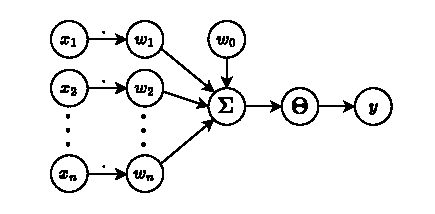
\includegraphics[width=0.75\textwidth]{../fig/background/Perceptron.pdf}
    \caption[Perceptron]{Architecture of the perceptron algorithm. Features $x_i$ are multiplied with their respective weights $w_i$ summed together with the bias term $w_0$ and passed through an activation function $\Theta$ to produce the output $y$.}
    \label{fig:perceptron}
\end{figure}
Functions mapping to values in the range $[0, 1]$, such as the step function or sigmoid functions, are used in classification tasks. Other (mostly) monotonic functions are used for activation in regression tasks. Due to their frequent invocation, computationally inexpensive functions like the Rectified Linear Unit (ReLU) are widely used in practice. The Gaussian Error Linear Unit (GeLU) converges to ReLU in the positive and negative limits, but smooths the transition around zero, ensuring differentiability over the entire domain. Some commonly used functions are depicted in \autoref{fig:activation_functions}. 
\begin{figure}[H]
    \centering
    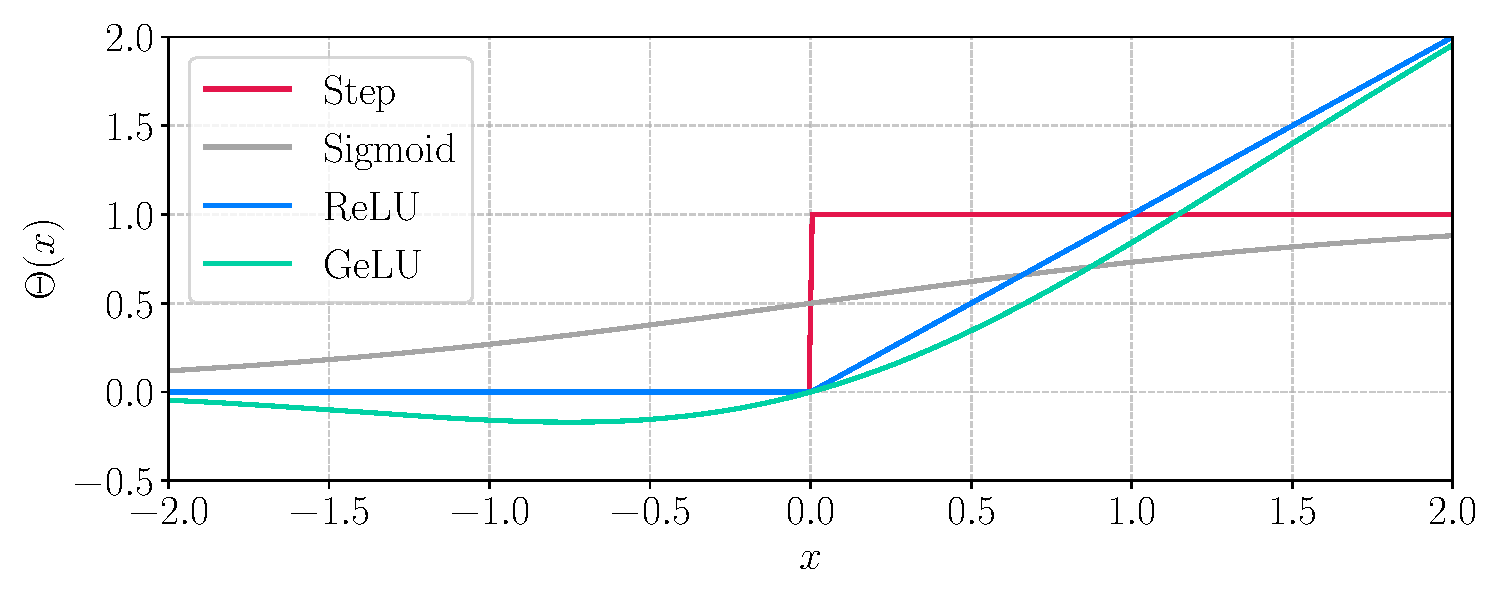
\includegraphics[width=0.8\textwidth]{../fig/background/activation_functions.pdf}
    \caption{Commonly used activation functions.}
    \label{fig:activation_functions}
\end{figure}
\subsection{Feed forward Networks: Multilayer Perceptron (MLP)}
\label{subsec:background_mlp}
Feed forward networks refer to a network architecture in which the outputs of the networks do not directly feed back into the inputs or any intermediate representations. Hence the input is exclusively fed forward through the network to produce the output. This way, there are no loops in the network's dataflow, allowing for training via the backpropagation algorithm. A Multilayer Perceptron (MLP) as shown in \autoref{fig:mlp} combines many perceptrons in layers. Data feeds into the input layer perceptrons which are each connected to every other perceptron in the first hidden layer. This connectivity is referred to as `fully connected' or `dense'. After several hidden layers, an output layer provides the output in the desired dimensionality and often without activation.\\
Each connection is associated with a weight that must be learned to enable meaningful predictions on unseen data. This learning process relies on backpropagation, which applies the chain rule iteratively to compute the gradient of the loss with respect to each weight, propagating from the output layer backwards through the network. While data flows forward through the network during prediction, the resulting loss propagates backward, guiding how the weights are adjusted. \\
\begin{figure}[H]
    \centering
    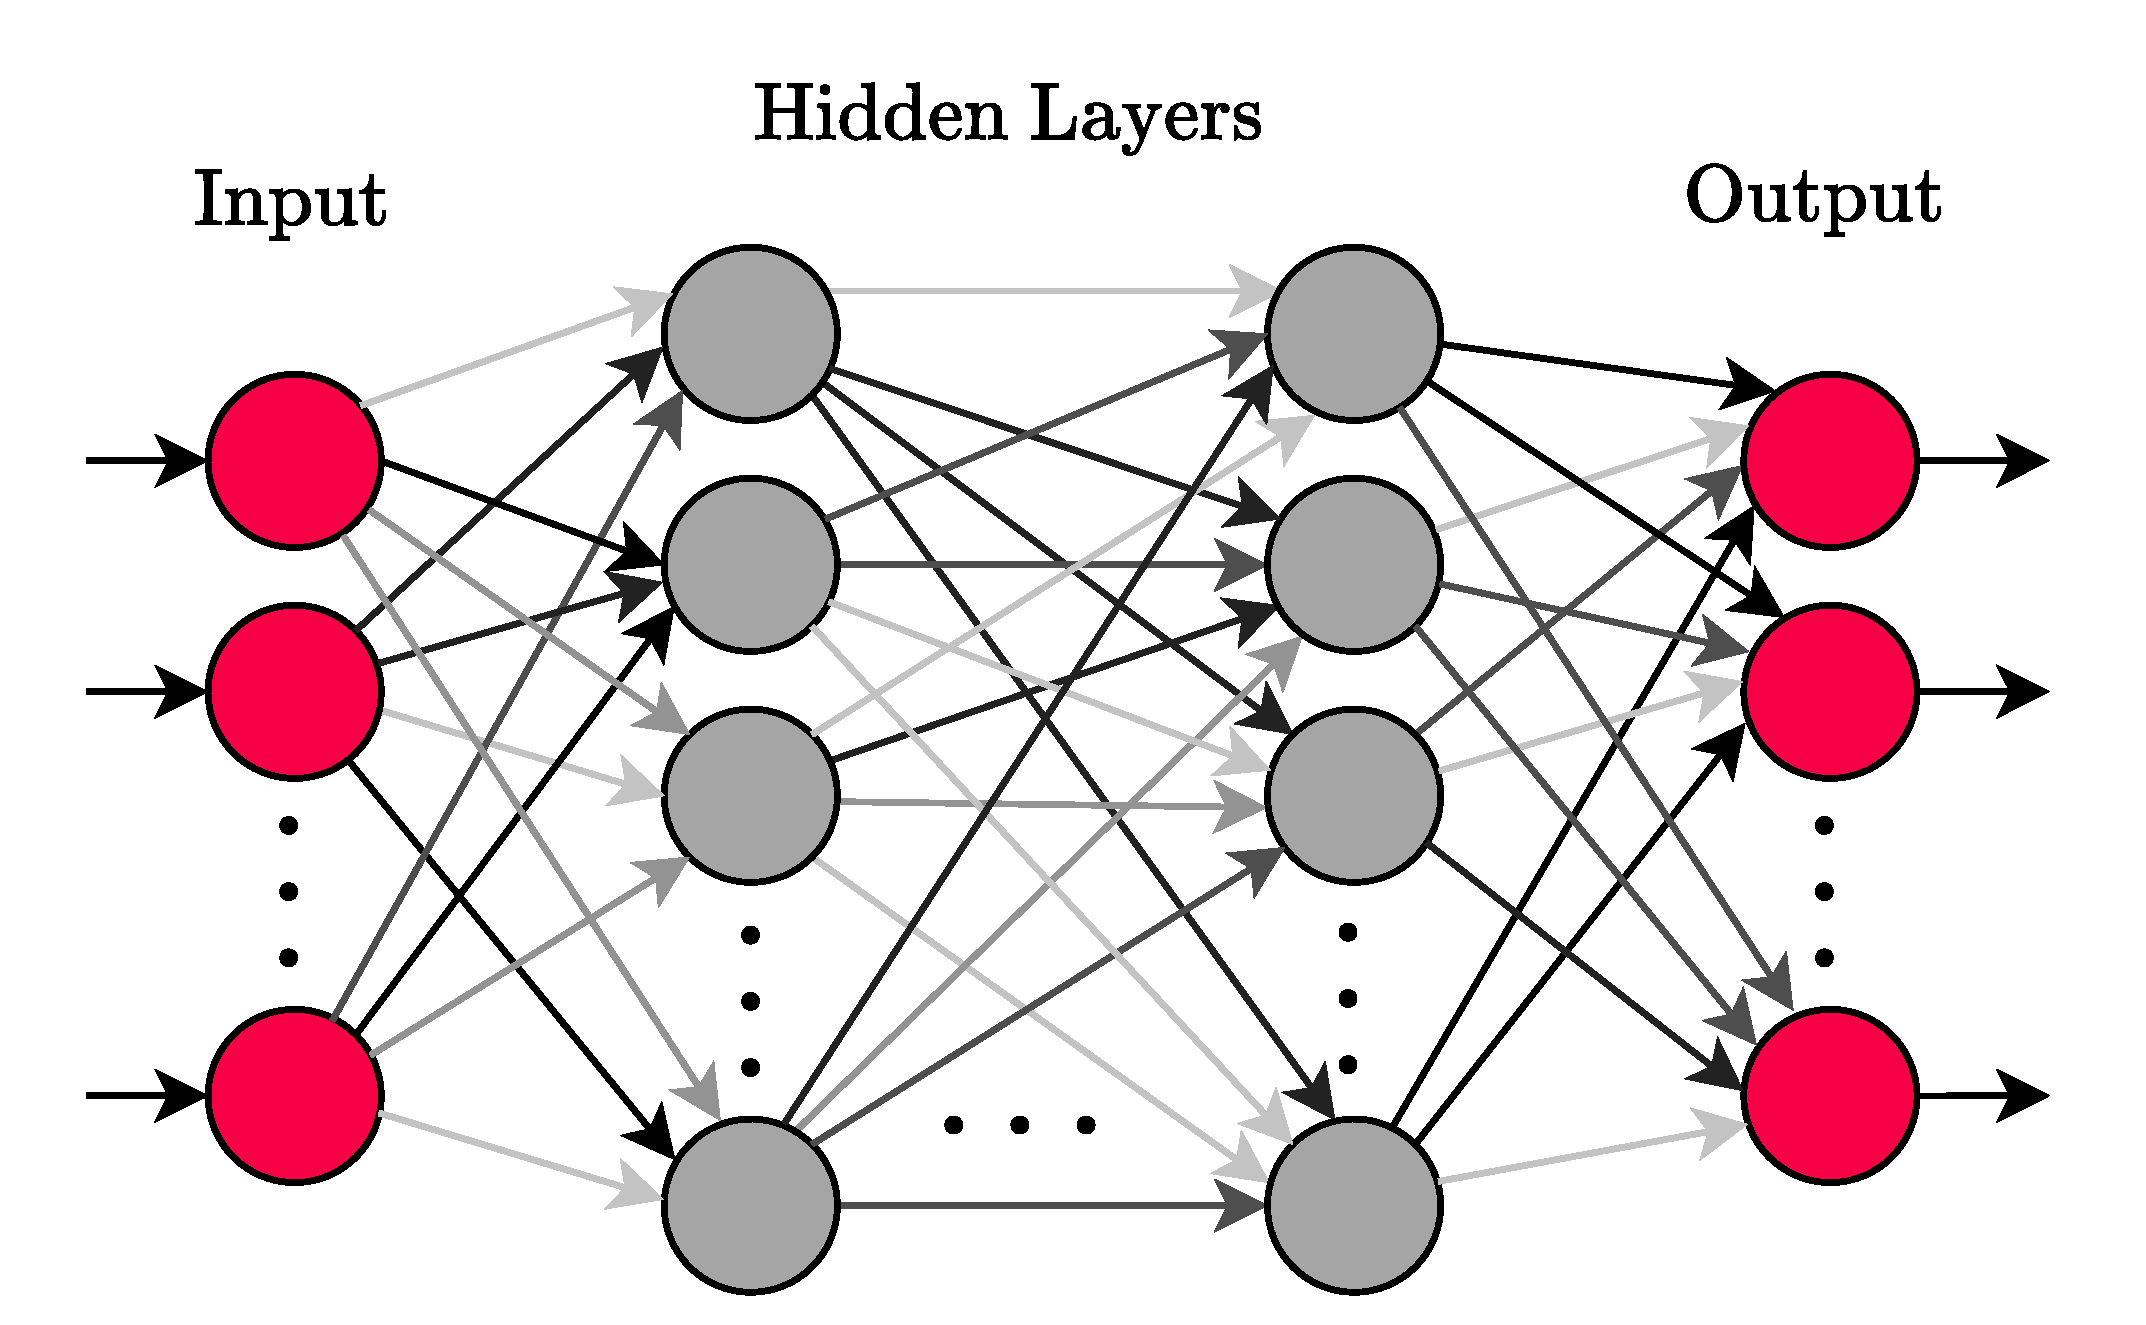
\includegraphics[width=0.6\textwidth]{../fig/background/MLP.pdf}
    \caption[Multilayer Perceptron]{Multilayer Perceptron with fully connected layers. Different shades of gray represent weights between perceptrons.}
    \label{fig:mlp}
\end{figure}

Similar to regression, regularization may also be added in various places. Besides $L_1$ or $L_2$ penalities, which can be easily added to the loss function, dropouts offer another, neural network-specific way of regularization. During training, it randomly sets outputs of perceptrons in the hidden layers to 0, thus deactivating the outgoing signal and reducing interdependence between perceptrons. 

\subsection{Graph Neural Network (GNN) / Message Passing Neural Nets (MPNN)}
\label{subsec:background_gnn}
Many problems cannot be simply mapped to a flattened input vector without losing information that is important for accurate predictions. Within the context of atomistic theories, a natural representation e.g. for a molecule may be attained by using a graph consisting of atoms as the nodes and edges between these nodes to represent interaction (e.g. bonds) between atoms. Learning features on graphs using a Graph Neural Network (GNN) is exploited in various fields and across different scales, from large protein structurs in DeepMind's Alphafold \parencite{ref:alphafold} down to molecular features such as energy, polarization and charge density in computational quantum chemistry. For the latter, the term `Message Passing Neural Nets' (MPNN) was coined by Glimer et al. in \parencite{ref:gilmer2017neural}.

An abstract representation of a MPNN is depicted in \autoref{fig:gnn_background}. Data, such as colour in the concrete example, is encoded in the nodes of a graph. For many use cases, separate encoder functions or even MLPs may be suitable for the encoding of various features into a feature vector for a given node or edge. For molecules, these might include atomic number, electronegativity or even overlap matrix elements. After initialization of the graph, the MPNN iteratively updates the nodes feature vector for several message passing rounds. 
\begin{figure}[H]
    \centering
    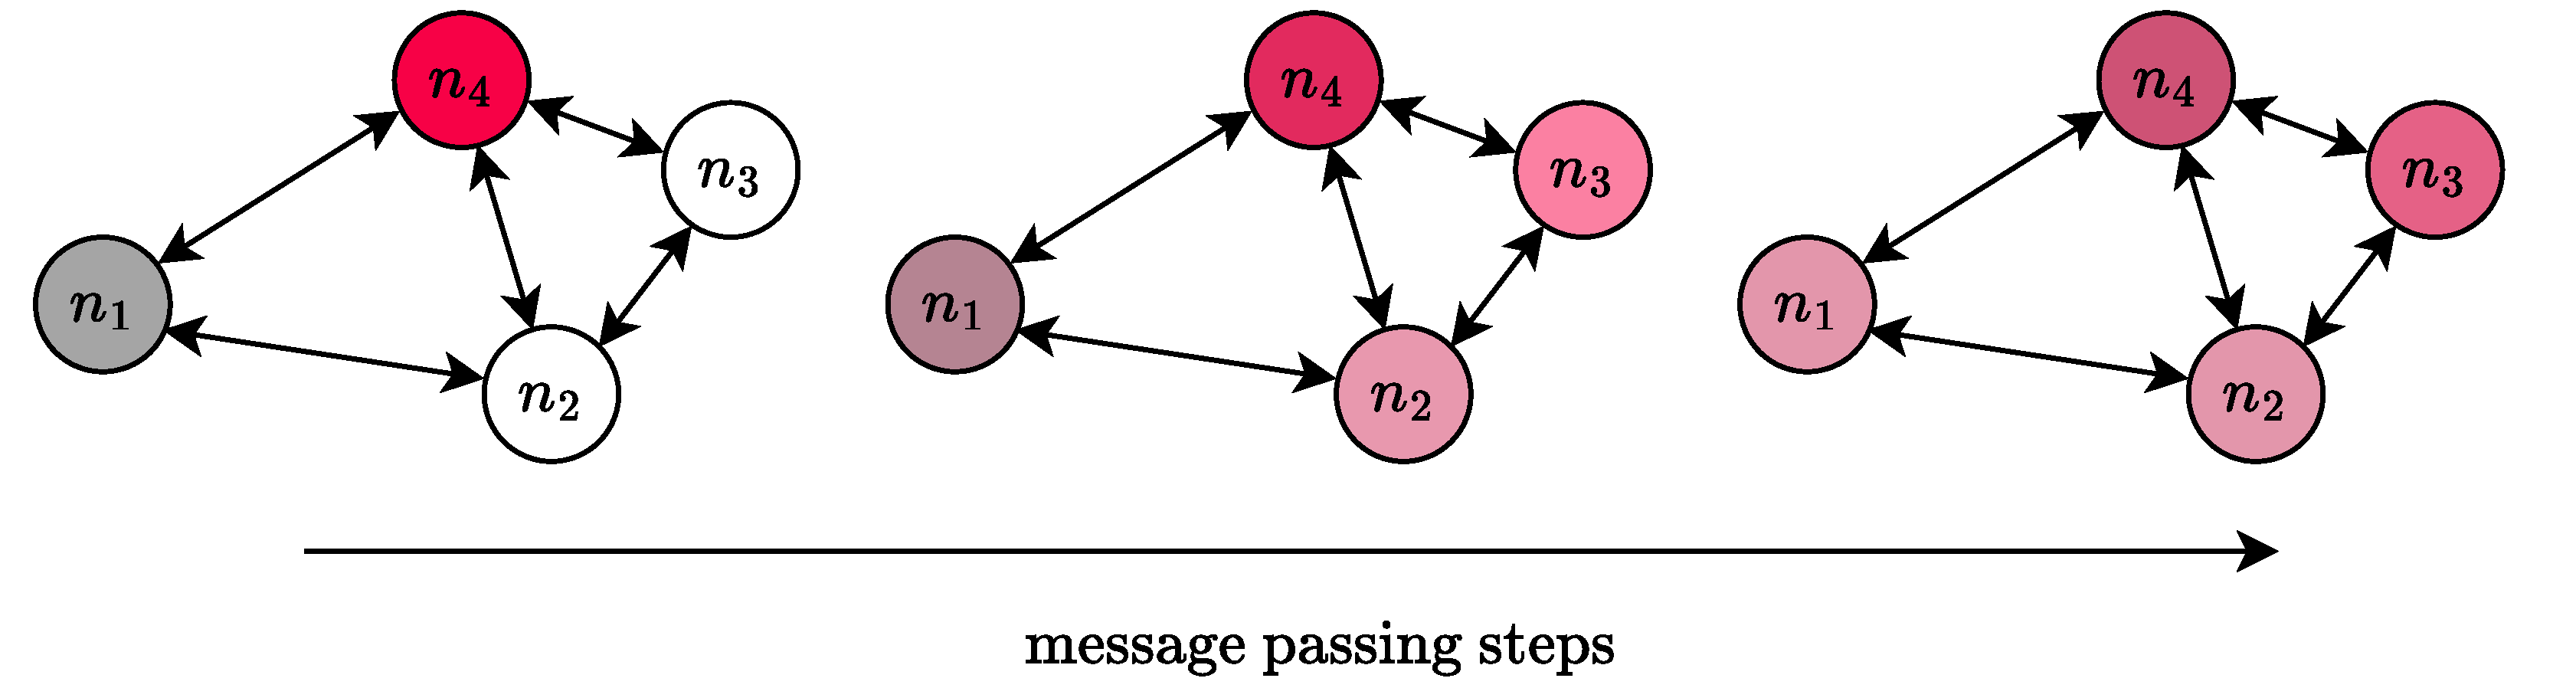
\includegraphics[width=\textwidth]{../fig/background/GNN.pdf}
    \caption[Schematic Message Passing Neural Net]{Schematic representation of message passing in a bidirectionally connected graph. Node colours influence neighbours which aggregate neighbour colours and updates own colour via leaned update function each step.}
    \label{fig:gnn_background}
\end{figure}
For every round, all nodes send a message containing their feature vector (or a derived representation) to all their neighbours. The node $n_1$ in \autoref{fig:gnn_background} sends its colour to its neighbours $n_2$ and $n_4$. After all messages have been sent, every node aggregates the received message via a permutation invariant function. In the example, this is simply the average of the received colours. Finally, a learned update function changes the node's feature vector based on the aggregated message and the current feature vector. After several rounds of message passing, which allow information flow between nodes not directly connected to each other, the final graph representation can be used to predict various properties.\\
Decoders essentially invert the encoder's process to extract either node-level features (e.g. atomic energy, partial charge or node colour in \autoref{fig:gnn_background}) or graph-level properties such as total energy, polarizability or electric dipole moment.

\subsection{Neural Network Training and Hyperparameter Tuning}
\label{subsec:background_ml_training}
Training neural networks and tuning their hyperparameters are crucial steps to ensure models learn meaningful patterns and generalize to unseen data. This section outlines the standard training workflow and introduces two hyperparameter optimization methods employed in this thesis: Bayesian search and Hyperband.

\textbf{Network Training}\\
Training begins with the random initialization of network weights. Input data is processed in the network in batches (e.g. 16, 32 or 64 input samples). For each batch, the network performs a forward pass to generate predictions and compute a loss value using the loss function. Backpropagation then calculates gradients of the loss with respect to each weight in the network. The weights are updated using an optimization algorithm, which adjusts the weights in the direction that reduces the loss. This cycle (forward pass, loss computation, backpropagation) repeats for multiple epochs, where one epoch corresponds to one full pass through the training dataset. \\
Key hyperparameters influencing training dynamics and overall model performance include the learning rate, batch size, number of epochs, and network architecture: the number of layers, neurons per layer, and activation functions.

\textbf{Hyperparameter Tuning}\\
Hyperparameter tuning explores the space of settings to identify combinations that yield the best results. An exhaustive search over all possible combinations is typically infeasible and not possible for continuous-valued hyperparameters. Within this thesis, two approaches will be used: Bayesian search and Hyperband tuning.

\textbf{Bayesian Search Tuning}\\
Bayesian search constructs a surrogate probabilistic model mapping hyperparameters to performance. After evaluating a set of configurations, it updates this model to predict promising regions in hyperparameter space. By sampling where improvement is most likely, it outperforms random or grid search in efficiency and convergence speed.

\textbf{Hyperband Tuning}\\
Hyperband tuning methods combine the exploratory power of random search with early stopping to efficiently allocate resources only to promising hyperparameter configurations. It starts with many random configurations, trains each for a few epochs, and discards the worst performers. The top configurations receive additional resources in subsequent rounds. This process is repeated until a certain budget is reached or a maximum number of configurations have been evaluated. This optimization strategy can be fully parallelized, allowing independent evaluation of configurations and fast identification of strong candidates. 
\newpage
\section{QM9 dataset}
\label{sec:dataset}
Dataset selection for training is dominated by two practical considerations:
\begin{enumerate}
    \item Cost per sample: Time savings through faster convergence are especially relevant for larger systems where the number of SCF iterations and the number of integrals to be calculated are large. Stated differently, it is of little interest to optimize guessing methods for small systems that converge nearly instantly on conventional hardware. 
    \item Fixed I/O size: Most ML models are constrained to a constant input and output size. 
\end{enumerate}

The QM9 dataset \parencite{ref:data_qm9, ref:article1_qm9,ref:article2_qm9} ticks both of these two boxes. It offers a variety of molecules from as little as three constituent atoms up to 29 atoms. Additionally, there are large enough chunks of constitutional isomers to train models on these subsets of same sized matrices. The distribution of molecules by atom count with the predominant constitutional isomers is shown in \autoref{fig:method_qm9_overview}.
\begin{figure}[H]
    \centering
    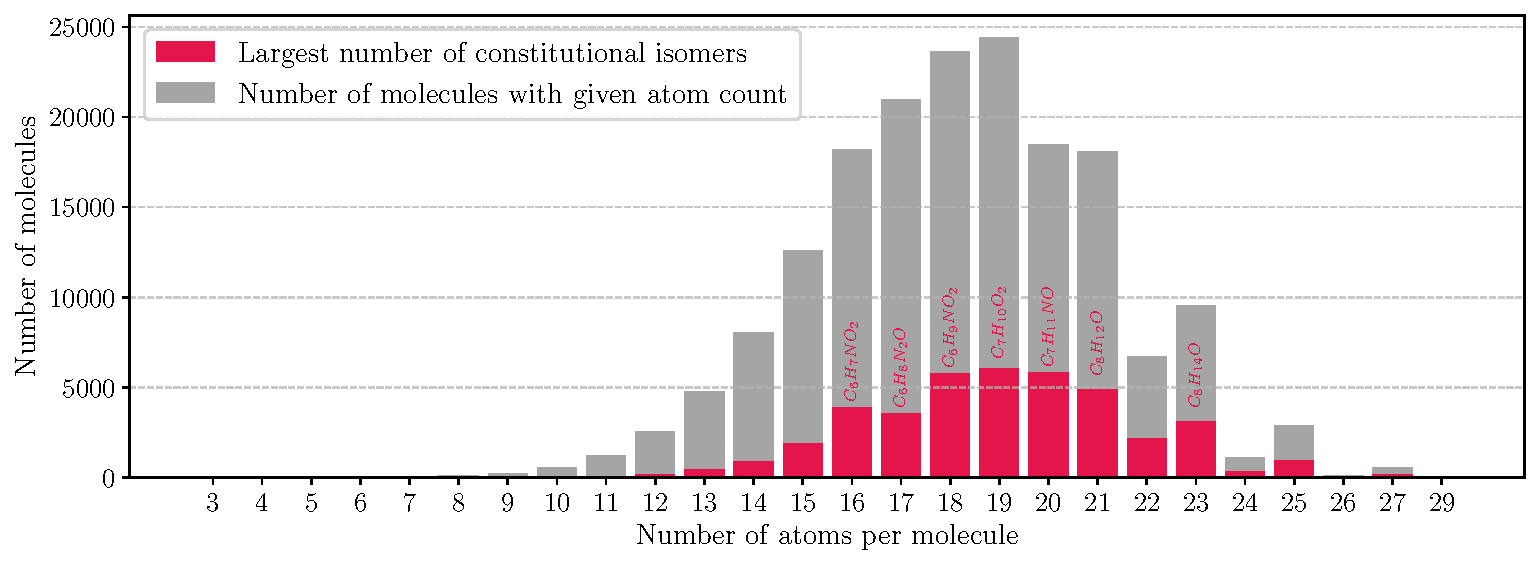
\includegraphics[width=0.85\textwidth]{../fig/qm9_general/qm9_overview_stacked_bar.pdf}
    \caption[QM9 dataset overview]{Overview of the QM9 dataset. The dataset contains $134,000$ molecules with up to nine second row elements (\ch{C}, \ch{O}, \ch{N}, \ch{F}). Large groups of constitutional isomers are present (largest depicted in red).}
    \label{fig:method_qm9_overview}
\end{figure}
%! Trajectories moved to Application chapter!
